% Historique du sujet
% Introduction théorique
% Application dans la vie courante
Les filtre passe-haut et passe-bas sont utilisés dans les domaines de retouche visuelle et sonore comme dans des amplificateurs audios (écouteurs et enceintes) et dans les circuits de communication. Grâce à sa propriété sélective qui ne laisse passer qu'une partie des fréquences, ces filtres permettent d'atténuer le bruit (avec un filtre passe-bas), ou bien de l'amplifier (filtre passe-haut). \\
Par exemple, dans la retouche de photos et vidéos, un filtre passe-haut permettrai d'obtenir une image plus nette. En utilisant un filtre passe-haut puissant, nous obtenons la transformation suivante :

\begin{figure}[H]
  \centering
    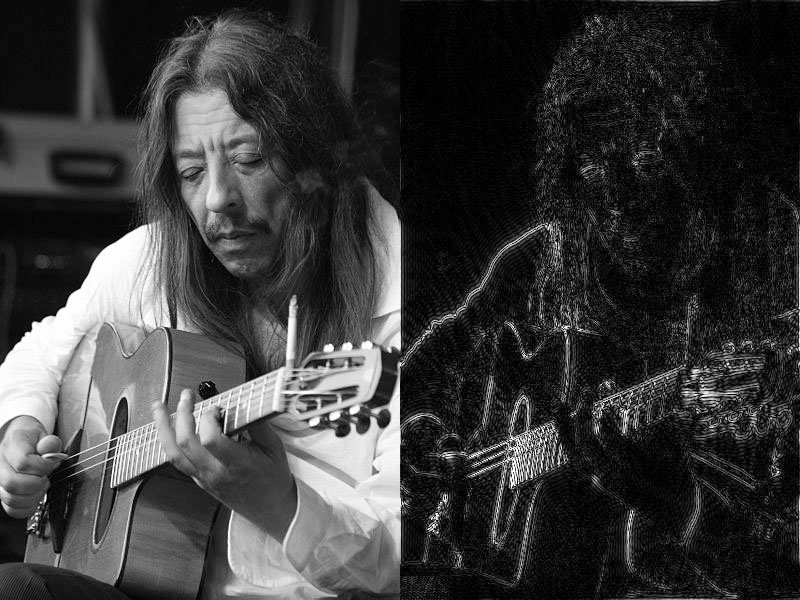
\includegraphics[width=0.25\textwidth]{Highpass_picture.jpg}
    \caption[Avant et après l'application d'un filtre passe-haut]{Avant et après l'application d'un filtre passe-haut \footnotemark}
\end{figure}
\footnotetext{Issu de \href{https://fr.wikipedia.org/wiki/Filtre_passe-haut}{Wikipédia - Filtre passe-haut}}

Au contraire, les filtres passe-bas permettent de lisser des objet ou des figures. Avec un filtre puissant nous pouvons effectuer la transformation suivante: 

\begin{figure}[H]
  \centering
    
\includegraphics[width=0.25\textwidth]{Lowpass_picture.jpg}
    \caption[Avant et après l'application d'un filtre passe-bas]{Avant et après l'application d'un filtre passe-bas \footnotemark}
\end{figure}
\footnotetext{Issu de \href{https://fr.wikipedia.org/wiki/Filtre_passe-bas}{Wikipédia - Filtre passe-bas}}

Le filtre passe-bas est aussi utilisé afin d'atténuer le bruit dans le contexte d'une transmission sonore par exemple. Ces filtres permettent de sélectionner une partie d'image ou de son et de la modifier comme voulu dans le but d'obtenir un résultat souhaité. \\

Pour faire cela, ces filtres ne laissent passer qu'une partie des fréquences et atténuent les autres. L'utilisation des deux filtres (passe-haut et passe-bas) se nomme un filtre passe-bande. Physiquement, un filtre passe-haut est constitué d’un condensateur (plus la fréquence est élevée, plus il se charge et décharge vite ce qui donne à la limite comme si le courant passait sans problème) suivi d’une résistance, et le filtre passe-bas d'une résistance et d'une \textit{self} (ou bobine, et plus la fréquence est élevée, plus la variation du courant est grande est plus l'auto-induction réduit celui-ci).\\

C'est uniquement à partir d'une certaine fréquence, que ces filtres feront effet. Celle-ci se nomme une fréquence de coupure.
Dans le cas du filtre passe-haut, les fréquences inférieures à sa fréquence de coupure $f_c$ sont atténuées, et les fréquence plus haute seront mise en valeur.
Au contraire, le filtre passe-bas atténue les fréquences supérieurs à sa fréquence de coupure $f_c$ pour valoriser les fréquence plus basse.

\begin{figure}[H]
  \centering
  \begin{minipage}[b]{0.4\textwidth}
    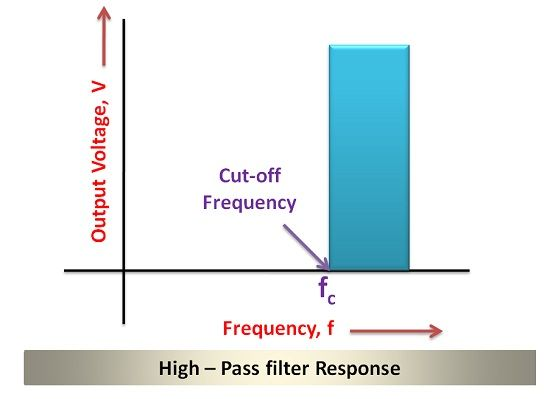
\includegraphics[width=\textwidth]{HFP-response.jpg}
    \caption[Fonctionnement d'un filtre passe-haut]{Fonctionnement d'un filtre passe-haut}
  \end{minipage}
  \hfill
  \begin{minipage}[b]{0.4\textwidth}
    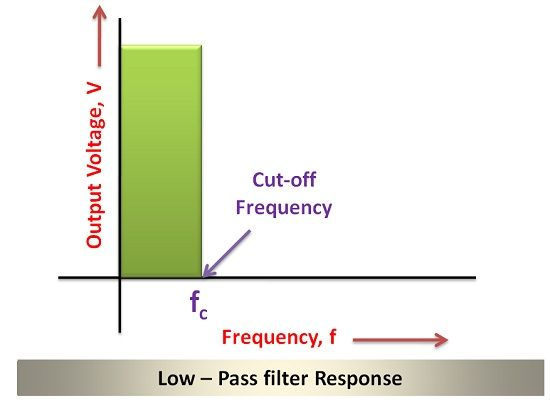
\includegraphics[width=\textwidth]{LPF-response.jpg}
    \caption[Fonctionnement d'un filtre passe-bas]{Fonctionnement d'un filtre passe-bas \footnotemark}
  \end{minipage}
\end{figure}
\footnotetext{Issu de \href{https://electronicscoach.com/difference-between-high-pass-and-low-pass-filter.html}{https://electronicscoach.com/difference-between-high-pass-and-low-pass-filter.html}}

Comme nous pouvons le voir sur les images, le voltage $V$ monte ou descend de manière verticale à partir d'une certaine fréquence $f_c$. En effet, dans le cas d'un filtre passe-haut parfait, la tension atteindra instantanément son maximum. Or, en réalité, cela n'est pas tout a fait le cas. Avec une utilisation une variation régulière (sinusoïdale) de la tension, nous pouvons nous attendre cela:

% Utilisation d'une sinusoidale pour avoir un courant variant réguliérement -> observe le filtre par l'aténuation de la tension / du courant selon la fréquence (par le passage dans la bobine ou le condensateur)
% note pour demarche: Du a l'attenuation, il ets possible que la courbe n'atteigne pas son maximum
\begin{figure}[H]
  \centering
    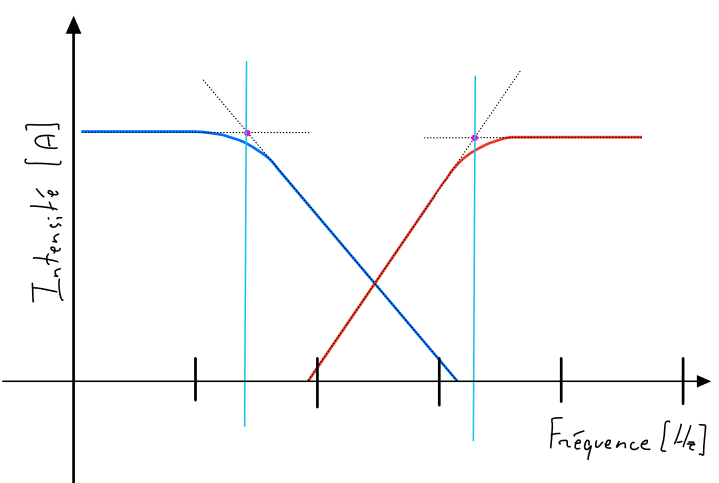
\includegraphics[width=0.4\textwidth]{phy_FPB-FPH.PNG}
    \caption{Graphe des filtres passe-haut et passe-bas}
\end{figure}

En bleu la réaction du filtre passe-bas, et en rouge celle du passe-haut. Une fois qu'ils atteignent leur fréquence de coupure (en cyan), nous observons une augmentation / diminution progressive de l'intensité.\\

Comme la variation de la tension est régulière, la tension électromotrice se présente comme suit:
$$
    U(t) = \widehat{U} \sin(\omega \cdot t + \phi_1)
$$
Tel que $U(t)$ la tension en fonction du temps, $\widehat{U}$ la tension maximale, $\omega$ la pulsation imposée par le générateur et $\phi_1$ indique que $U(t)$ n'est pas forcément nulle lorsque t=0.

\subsection{Le circuit \textit{RC}}
Le circuit \textit{RC} agit comme un filtre passe-haut. Ce dernier consiste à placer une résistance $R$ et un condensateur $C$ en série, puis y faire passer un courant alternatif.\\
Le courant produit est donné par:
$$
    I(t)=\widehat{I} \sin(\omega \cdot t + \phi_1) \hspace{0.5cm} \text{avec} \hspace{0.5cm} \widehat{I} = \frac{\widehat{U}}{Z}
$$
Tel que $I(t)$ l'intensité en fonction du temps, l'intensité maximale $\widehat{I}$, qui dépend de l'impédance (l'opposition d'un circuit électrique au passage d'un courant alternatif sinusoïdal \footnote{Selon \href{https://fr.wikipedia.org/wiki/Imp\%C3\%A9dance_(\%C3\%A9lectricit\%C3\%A9)}{Wikipédia - L’impédance (électricité)}}) $Z$ déterminée par la résistance $R$, la charge électrique $C$ et $\omega$ la pulsation imposée par le générateur:
$$
    Z = \sqrt{R^2 + (\frac{1}{\omega C})^2}
$$

et le déphasage $\phi_1 - \phi_2$ lié par:
$$
    \tan(\phi_1 - \phi_2) = -\frac{1}{\omega R C}
$$


\subsection{Le circuit \textit{RL}}

Le circuit \textit{RL}, consiste à placer une résistance et une self $L$ (ou bobine) en série aux bornes d'un générateur de tension alternatif. Ce circuit fait office de filtre passe-bas.\\
Comme pour le circuit $RC$, le courant est de la forme:
$$
    I(t)=\widehat{I} \sin(\omega \cdot t + \phi_1) \hspace{0.5cm} \text{avec} \hspace{0.5cm} \widehat{I} = \frac{\widehat{U}}{Z}
$$
A la différence que l'impédance est déterminée par:
$$
    Z = \sqrt{R^2+(\omega L)^2}
$$
et le déphasage $\phi_1 - \phi_2$ par:
$$
    \tan(\phi_1 - \phi_2) = \frac{\omega L}{R}
$$
Lors de cette expérience nous avons introduit un $\Delta t$ tel que: $\Delta t = \frac{\phi_2 - \phi_1}{\omega}$, afin de mesurant l'écart entre $\widehat{I}$ et $\widehat{U}$.

\begin{figure}[H]
  \centering
    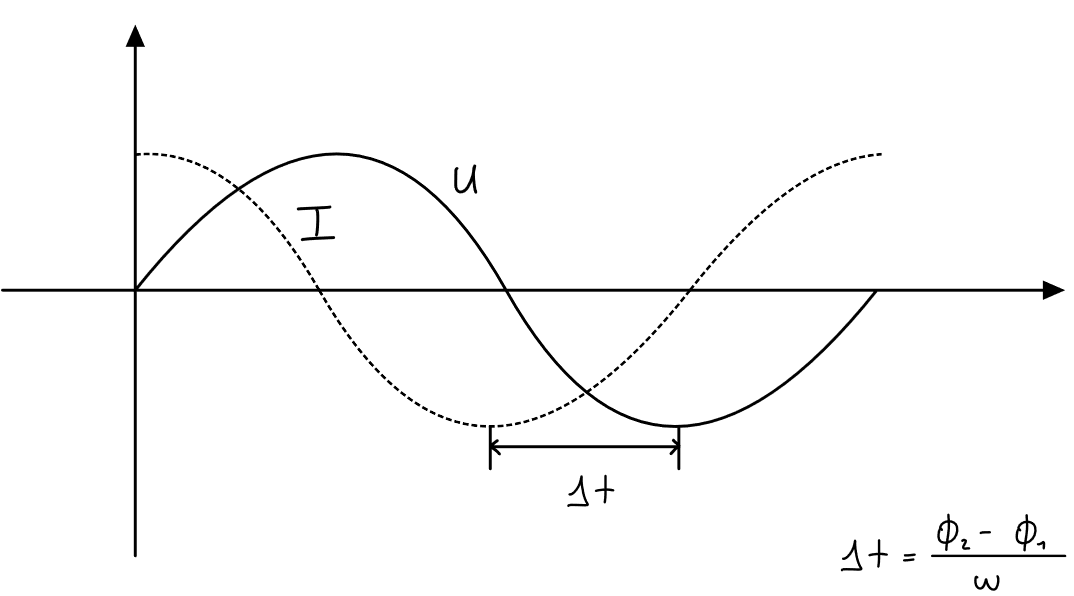
\includegraphics[width=0.5\textwidth]{phy_delta-t.PNG}
\end{figure}